\if0
先述のHL7などの共通の規格が活用されていない現実があるので,
いろんな規格の差を吸収できるようなアプリは需要があると考える.
三重県にこのような医療ネットワークを実現するためのたたき台として
本研究では開発を進めた.
\fi



\subsection{SQL版について}
  特定の病気にかかっている複数人の患者の医療情報が記載された
  エクセルファイルを医療関係者から提供していただいた.
  医療情報として検査値,投薬についての情報などが記載されていた.
 このエクセルのデータのみを受け付けるアプリをDjangoで開発した.

  検査値,投薬についての情報を患者の認可のもとで収集し,
  SQLデータベースに保存する.
  患者に認可をされた医療関係者は情報の参照,書き込みが可能となる.

  このサービスを実現するために後述する機能を実装した.

  本研究ではユーザとして患者と医療関係者の2つの立場があることを想定している.
  ユーザモデルは二者を区別できるように実装し,
  二者で異なる使い方ができるようにした.

  具体的には患者は自身の情報を誰にも阻害されずに閲覧でき,
  医療関係者は認可があれば複数人の患者の情報を操作することができる.



\subsection{SQL版が有する機能}
  \subsubsection{データ入力}
    SQLのテーブルに則った検査値と投薬についての情報の
    CSVファイルから医療情報をデータベースへ入力することができる.

    \begin{figure}[htbp]
  		\begin{center}
  			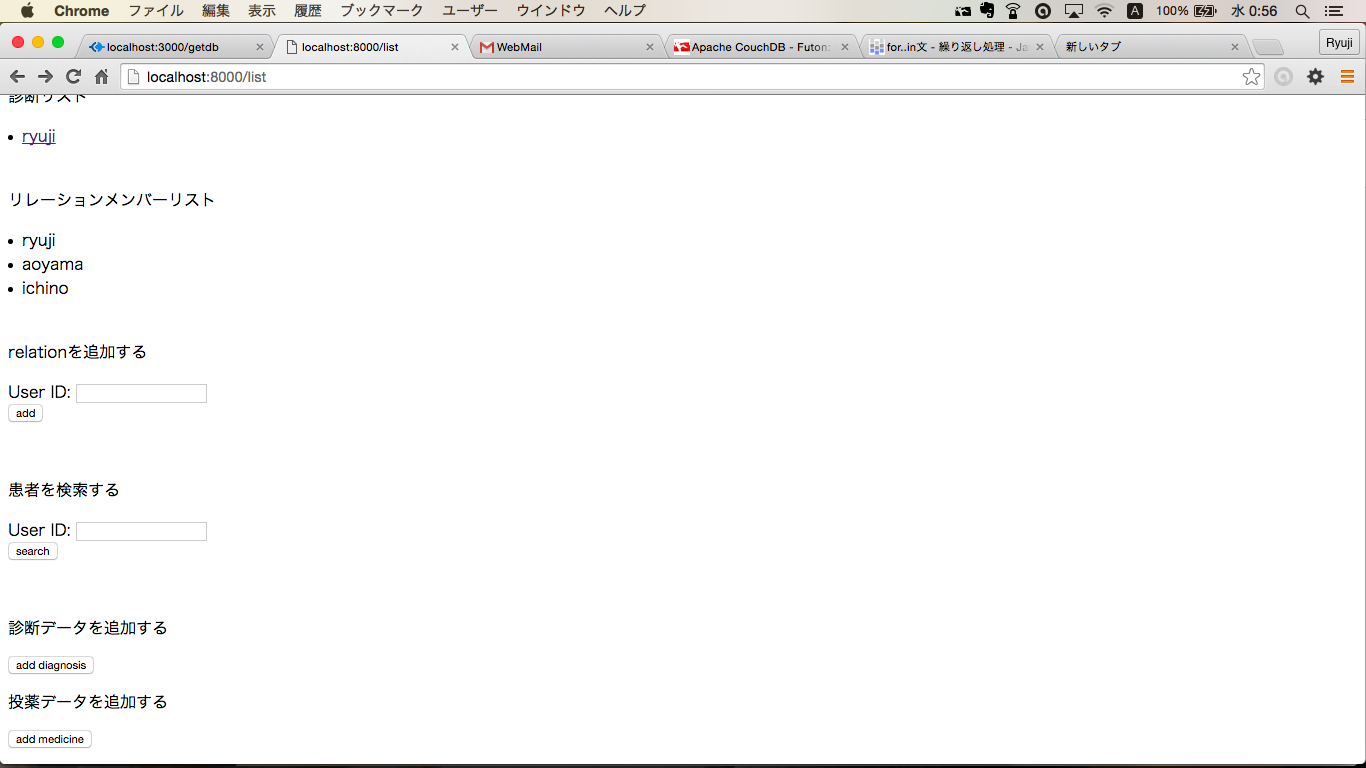
\includegraphics[width=5cm, bb=0 0 645 790]{./gazou/DjangoFileio.png} %よこたて
  		\end{center}
  		\caption{データ入力画面}
  		\label{DjangoFileio}
  	\end{figure}

  \subsubsection{データ閲覧}
    診断データは表にして、縦方向に診断項目,
    横方向に診断を行った日をとっている.
    空白部分はデータが入力されていない項目である.

    \begin{figure}[htbp]
      %\begin{center}
        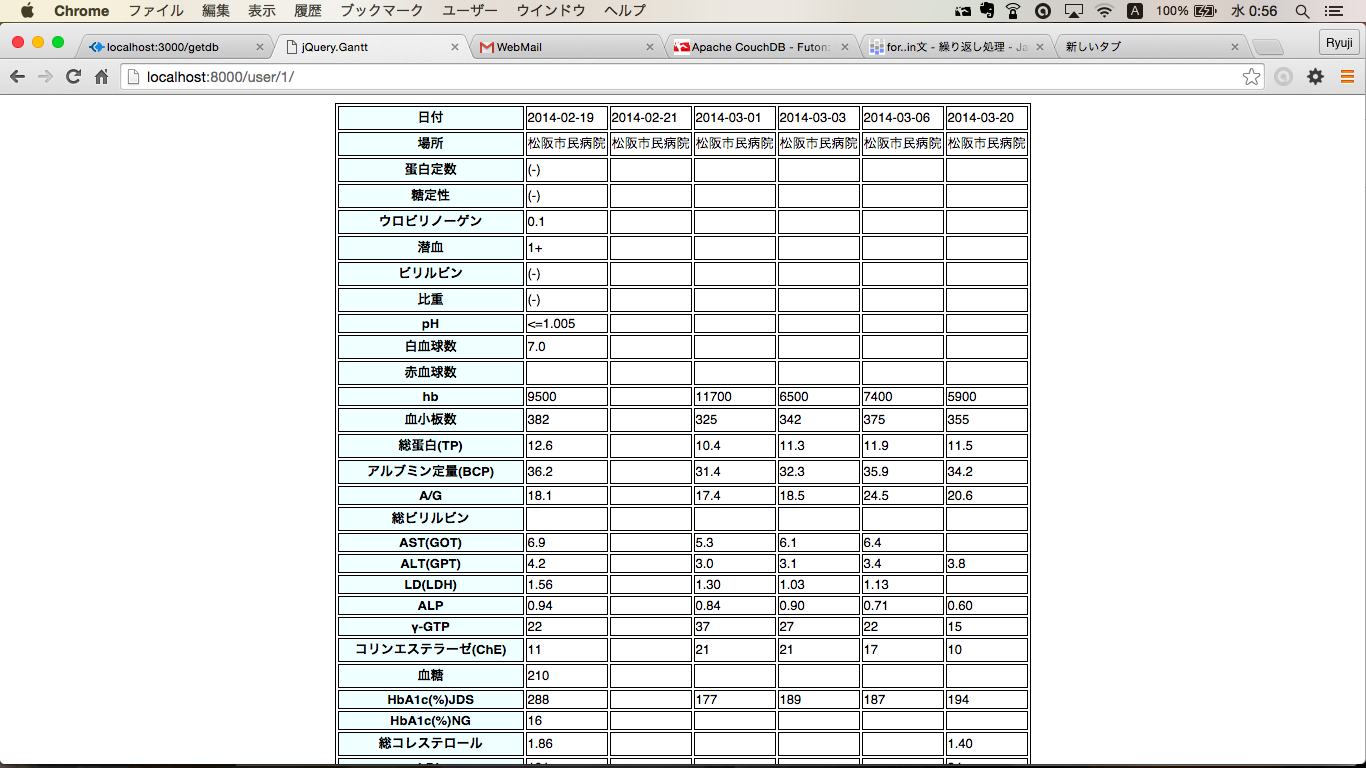
\includegraphics[width=5cm, bb=0 0 645 790]{./gazou/DjangoTable.png} %よこたて
      %\end{center}
      \caption{表によるデータ閲覧}
      \label{DjangoTable}
    \end{figure}

    \begin{figure}[htbp]

    投薬データはある薬をどれだけの期間服用しているかを
    わかりやすくするためにガントチャートのように表示している.
    これにより飲み合わせの薬を視覚的に見つけやすくすることができる.

    %\begin{center}
      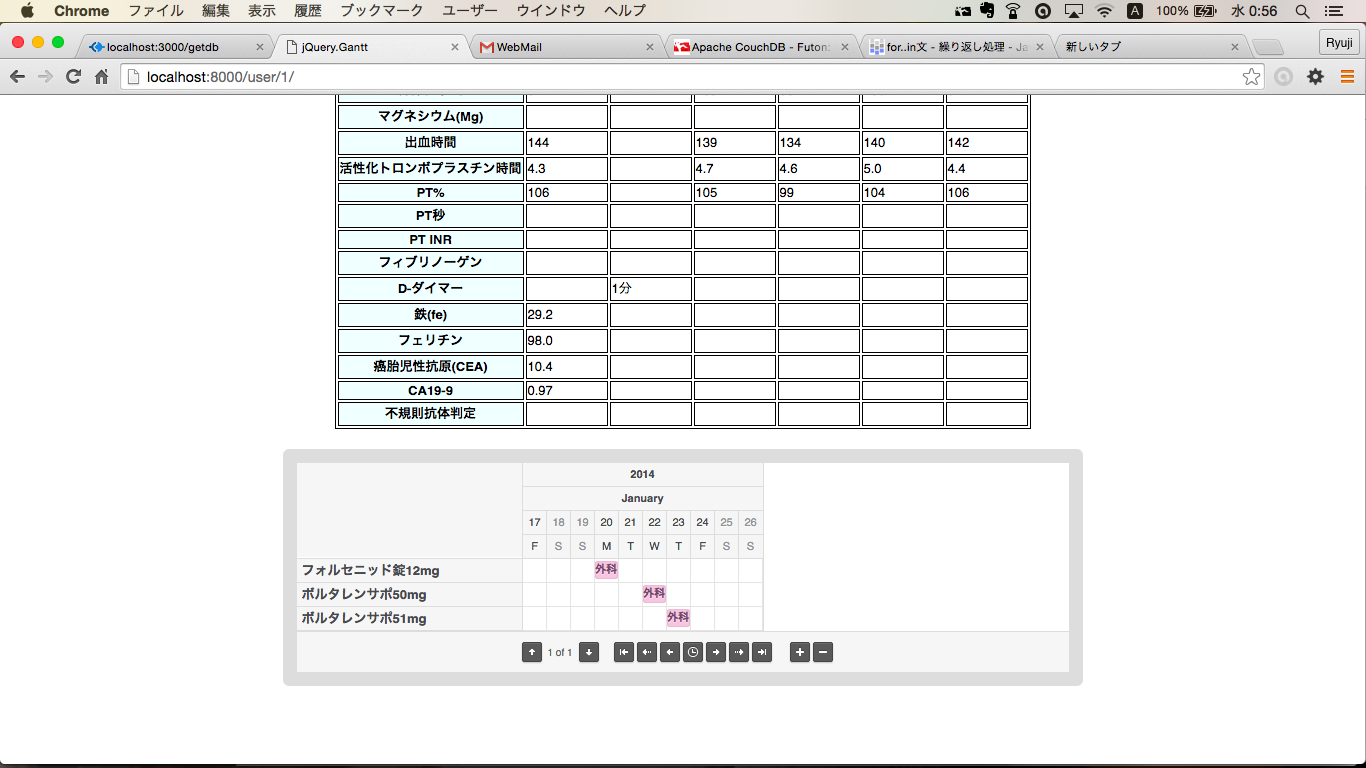
\includegraphics[width=5cm, bb=0 0 645 790]{./gazou/DjangoGantt.png} %よこたて
    %\end{center}
    \caption{ガントチャートによるデータ閲覧}
    \label{DjangoGantt}
  \end{figure}

  \subsubsection{権限の付与}
    患者の医療情報をどの医療関係者が操作することができるかを
    患者自身が選択する.
    認可には段階を設け,患者が意図する医療情報の利用を促す.
    具体的には,アクセス可能,読み込み可能と書き込み可能の
    3段階の認可を用意することである.
    これにより,患者のプライバシーを保護しながら
    医療情報を活用する.


\subsection{SQL版の課題とフィードバック}

  開発アプリのデモンストレーションによって得た医療関係者からの
  意見の中で研究課題として任意の検査項目の抽出が挙げられる.

  他の意見はインターフェース寄りの要望が多かった.
  例えば,表によるデータの表示に対するフィードバックとして,
  任意の検査項目にハイライトをつけてほしいといった内容であったが,
  本研究で工数を割くことができなかったため開発を見送った.


\subsection{NoSQL版の目標設定}
  医療の現場からは電子カルテや血圧計の出力ファイルとして
  様々なCSVファイルが出力される.
  また,電子カルテに関してはHL7で規格化されたファイルが
  出力できることもある.

  これらのファイルでの入力を入力を受け付けるWebアプリケーションを
  CouchDBを用いて実装する.


  デモンストレーションから得た課題を解決するには,
  まず入力データの言葉の揺れへの対応が必要となる.

  異なるフォーマットの入力データから,同じ意味の項目であっても,
  厳密に同じ言葉を項目名にとっていないことがある.
  ここでは便宜的に異なる項目名であるが同じ意味の項目の群を
  同義キーと呼ぶ.

  この同義キーを関連付ける機能を実装する.
  これにより,同義キーのうちのひとつが検索される際に,
  その同義キーの群の項目も検索結果として反映させる.





  \if0
  ドキュメントの数だけSQLデータベースのテーブルを用意する必要がある.
  データを検索する際にはjoinしてから.
  比べてNoSQLならガンガン入れて,
  データを出すときにだけKeyの関連づけをすればよい.
  NoSQLならSQLに比べてテーブルを用意する分の
  コストがはぶけてる(と言えるかな).
  \fi
